%!TEX root = thesis.tex

\chapter{Body Part Detection}
\label{ch:bodyparts}

To perform hand pose estimation of a person in a image, hands need to be localized in the image first. Hands are very deformable - they can have very different appearances and different orientations. Also hand size, hand shape and skin color can differ tremendously per person. This makes localization a  difficult task. 

One way to localize the hands is by searching for skin like colors in an image given a pre-calculated color profile. A generic skin color model based on average skin color has been constructed for this purpose\citep{Jones1999}. The problem with this method is that it fails when the skin color isn't `pure', for example when it is colored by a light source. Also, since the profile is very generic, it contains colors for many different skin colors. This introduces more false positives.

It is preferred to obtain the skin color of a person in a image from that image itself. This can be done by extracting the skin model from the face, which is much easier to detect than a hand.

This chapter describes how a skin model is created and how this is used to find the skin pixels in the image. These  skin pixels are clustered and labeled as left hand, right hand and head. 

\section{Skin Segmentation}
\label{sec:skinmodel}

\subsection*{Face localization}

\begin{figure}
  \center{}
    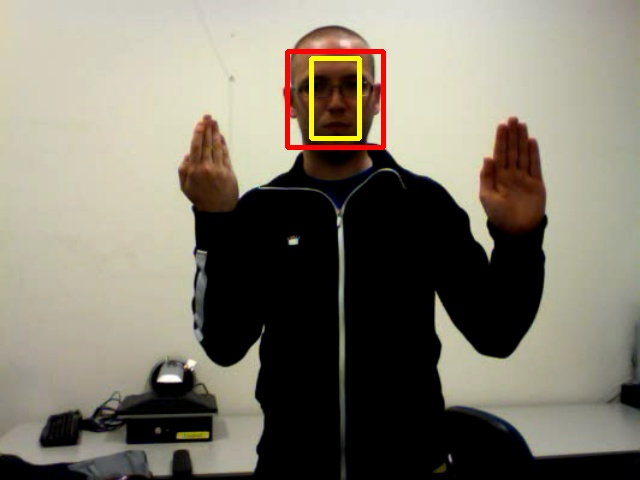
\includegraphics[width=0.6\textwidth]{figures/pipeline/detected.jpg}
  \caption{Face detection}
  \label{fig:face_detection}
\end{figure}

Finding faces in a image is a rather well solved problem. A face is easy to detect, since it is almost non-deformable. Different faces are quite similar looking at the most prominent properties, e.g. edges. People don't tilt their head often or not more than a couple degrees, which makes it even more easier to detect. Face detection can be done in a fast and robust way using a haar classifier, a boosted rejection cascade that is trained with Haar\-like wavelet\citep{Viola2001,Viola2004}. This  method doesn't rely on color information. The classifier is run over the image on different scales and positions with a score above a certain threshold are classified as face position, see \autoref{fig:face_detection} for an example. The red rectangle is the returned face location and size. This classifier is trained with traindata which also includes a small area of background, so this is also returned. Since we are only interested in the skin pixels a smaller sub-region is used for further processing. This sub square can be adjusted to minimize the influence of facial hair. 

Still, the face detection is a expensive operation. Fortunately, as a face doesn't move fast in a video sequence, a number of frames can be skipped which will free more computational time for other operations.

With the face location and size a skin color model of the user can be constructed.

\subsection*{Color Space Conversion}
Usually, pixel values of a image are stored in the Red, Green Blue (RGB) color space where colors are represented with combinations of these primary colors. The RGB representation of colors is not suitable for modeling skin color. The RGB color space represents not only color, but also luminance which is not a reliable measure for segmenting skin pixels\citep{Cai1999}.

When a subject is lighted by a light source with uniform hue distribution, the light doesn't change the hue or saturation of the subject. The only thing that will change is the luminance, which is changing because of the light source's intensity, distance or (self casted) shadow. Since we want to extract hand pixels independent of the illumination intensity, we can ignore this channel and only use the hue and saturation.

The luminance can be removed from the color space by transforming the color model to a chromatic color space. There are multiple chromatic color spaces, for example LAB, HSV and normalized RGB. No significant improvements are measured with a specific choice of these color spaces \citep{vsa03survey, Bradski1998}, so the HSV color space is used in the rest of this paper.

\begin{figure}[tb]
  \centering
\subfloat[HSV color space]{
	\label{fig:hsv}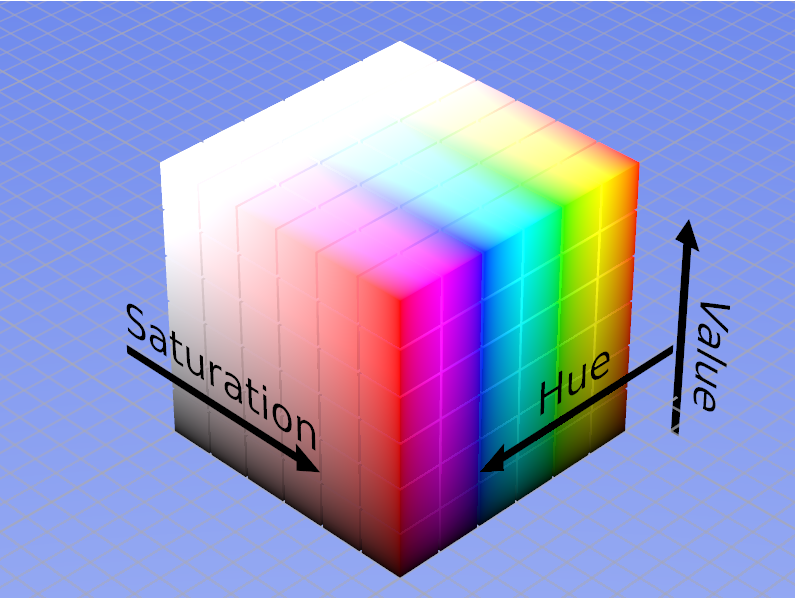
\includegraphics[width=0.45\linewidth]{figures/hsv2.png}
}
\hspace{0.01\linewidth}
\subfloat[RGB color space]{
	\label{fig:rgb}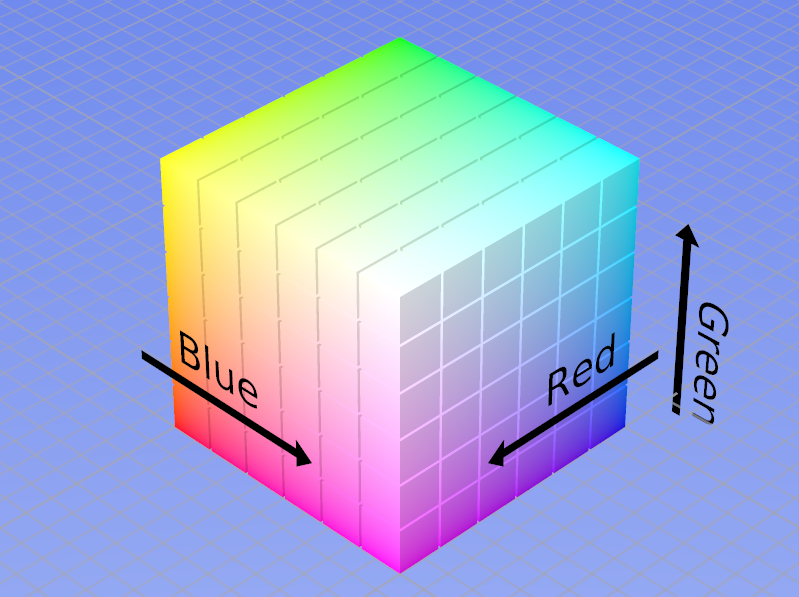
\includegraphics[width=0.45\linewidth]{figures/rgb.png}
}
  \caption{The RGB and HSV color space}
  \label{fig:colorspaces}
\end{figure}

HSV stands for hue (color), saturation (how concentrated the color is) and value (brightness). In practice a light source never has a uniform distribution and \emph{will} change the color of the subject. Fortunately, since we build a color model from the image itself, all skin pixels will change in the same way. 

The RGB color space is transformed into the HSV color space using the following equations:


\begin{eqnarray}
  V & \leftarrow & \max(R,G,B) \\
  S & \leftarrow & \left\{
  \begin{array}{l l}
    \frac{V-\min(R, G, B)}{V} & \quad \text{if $V \neq 0$} \\
    0 						  & \quad \text{otherwise} \\
  \end{array} \right.\\
  H & \leftarrow & \left\{
  \begin{array}{l l}
    \frac{60(G - B)}{S}     & \quad \text{if $V = R$} \\
    \frac{120 + 60(B-R)}{S} & \quad \text{if $V = G$} \\
    \frac{240 + 60(R-G)}{S} & \quad \text{if $V = B$} \\
  \end{array} \right.
\end{eqnarray}

Note that for computation reasons this a simplification of the real HSV color space. The real HSV colorspace is circular in the Hue dimension.

The input 3 channel RGB image is transformed into a 3 channel HSV image, after which the value channel is discarded. Using the detected face region of the hue and saturation channel a histogram can be constructed which will represent a statistical skin model.

\begin{figure}[tb]
  \centering
\subfloat[hue channel]{\label{fig:hue}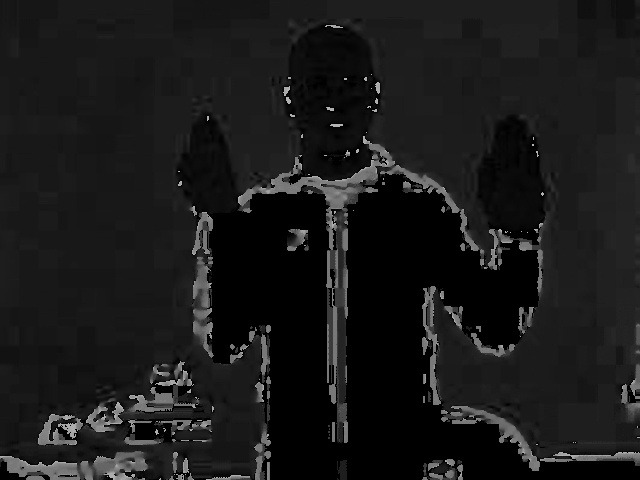
\includegraphics[width=0.3\linewidth]{figures/pipeline/hue.jpg}}
\hspace{0.03\linewidth}
\subfloat[saturation channel]{\label{fig:saturation}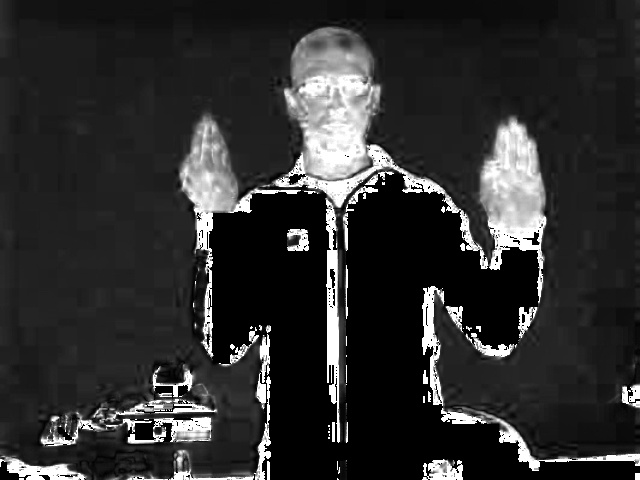
\includegraphics[width=0.3\linewidth]{figures/pipeline/saturation.jpg}}
\hspace{0.03\linewidth}
\subfloat[value channel]{\label{fig:value}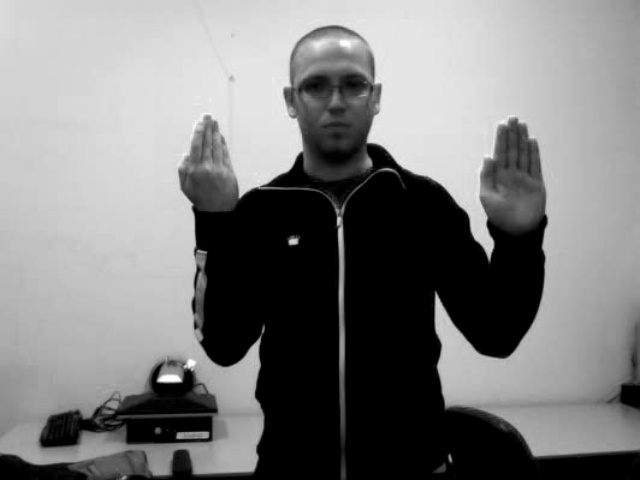
\includegraphics[width=0.3\linewidth]{figures/pipeline/value.jpg}}
  \caption{The HSV channels}
  \label{fig:hsvchannels}
\end{figure}




\subsection*{Statistical Skin Color Model}

\begin{figure}[tb]
    \center{}
    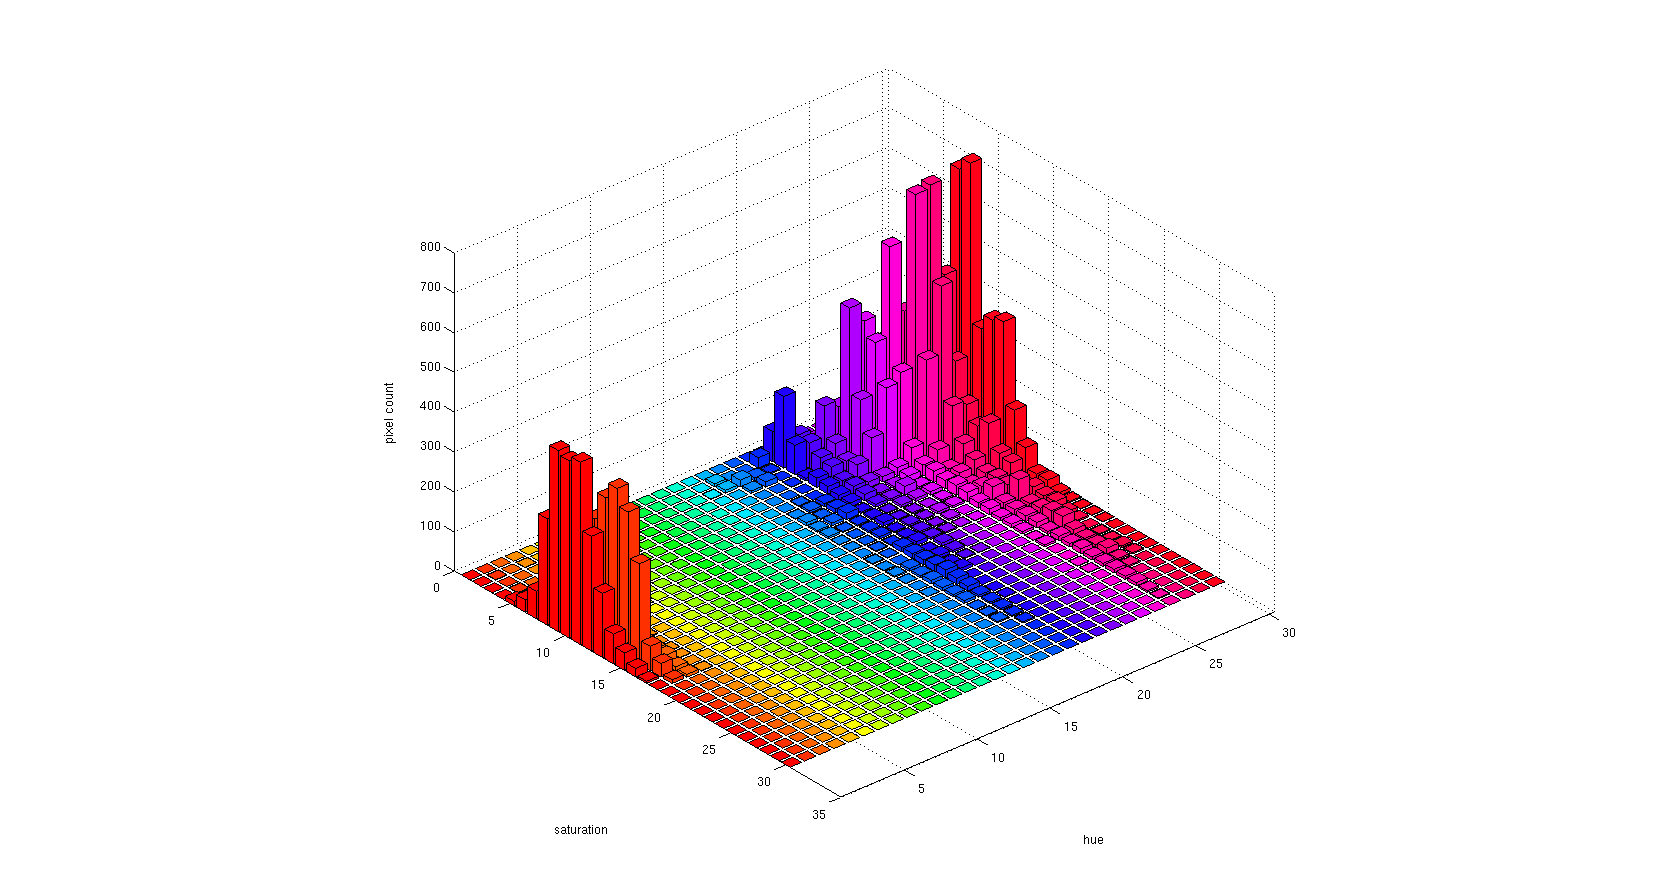
\includegraphics[width=1\textwidth]{figures/pipeline/histogram.png}
	\caption{A histogram of face pixels}
	\label{fig:histogram}
\end{figure}

There are multiple ways of constructing a statistical skin color model. The most conventional ways are a (mixture of) gaussian(s) or a histogram. 

The skin color model is represented in a 2 dimensional histogram, where the first dimension is Hue and the second is Saturation. The histogram is filled with the values from the detected face region. The histogram is normalized - all values are divided by the sum of all bins - to properly approximate the color density. This makes the histogram independent of the original image size, and each histogram bin value represents a `skin probablility'. \autoref{fig:histogram} is the histogram of a caucasian's skin color.

Manual experiments show that tweaking the number of bins doesn't have much effect, as long as the number of bins is not too high or not to low. Since for the storage of the values a 8 bit integer is used, a number of bins higher than 256 doesn't make sense. In all experiments mentioned in this paper a number of bins of 30 is used for both the hue and saturation.

\subsection*{Back Projection}

\begin{figure}[tb]
    \center{}
    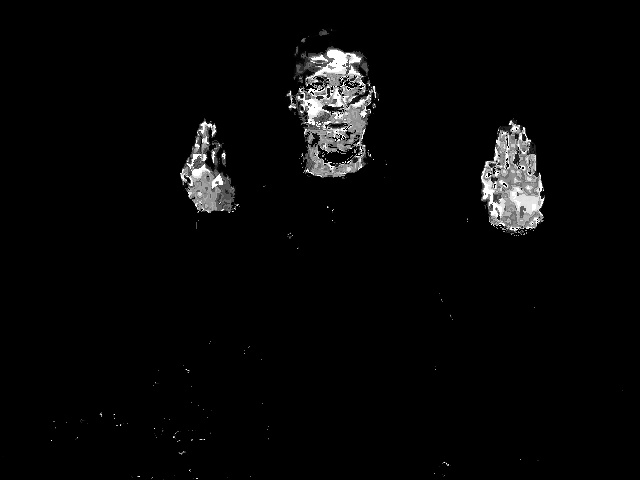
\includegraphics[width=0.5\textwidth]{figures/pipeline/backproject.jpg}
 	\caption{Backprojection}
	\label{fig:backproject}
\end{figure}


A back projection is the combination of an image and a histogram. The result is a new single channel image. All pixels in the input image are iterated and the corresponding bins are looked up in the histogram. The pixel in the same position in the new image is replaced with the value from the histogram. If the histogram is a skin color histogram, the resulting image will have high values for pixels that are skin-like pixels, and low values for other pixels. The result of the process can be seen in \autoref{fig:backproject}. Since the probabilities are very low the contrast of this image is enhanced so the maximum pixel value becomes pure white.


\subsection*{Smoothing}
Back projection can be quite noisy, which is caused by the rounding of values in the in the histogram and noise introduced by the camera. Thresholding this image will result in skin pixel groups with rough edges and a lot of holes, see \autoref{fig:threshold_noblur}. The noise can be reduced by smoothing the image. This way, the pixel value is replaced by the old value weighted with the surrounding pixel values. Using a gaussian kernel with a high $\sigma^2$ gives a good result, see \autoref{fig:blurred}.

\begin{figure}[tb]
    \center{}
 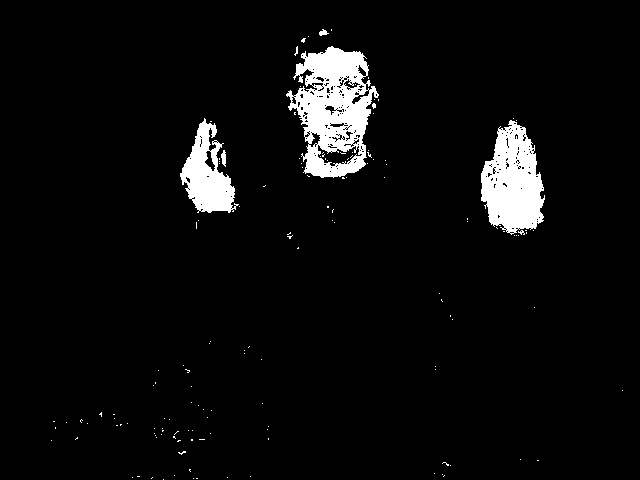
\includegraphics[width=0.5\textwidth]{figures/pipeline/thresholded_noblur.jpg}
	\caption{Thresholded image without blur preprocessing}
	\label{fig:threshold_noblur}
\end{figure}

\begin{figure}[tb]
    \center{}
    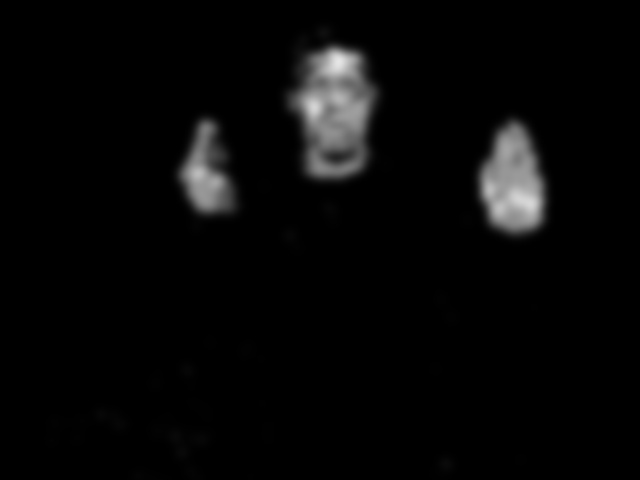
\includegraphics[width=0.5\textwidth]{figures/pipeline/blurred.jpg}
	\caption{Blurred image}
	\label{fig:blurred}
\end{figure}


\subsection*{Threshold}

\begin{figure}[tb]
    \center{}
    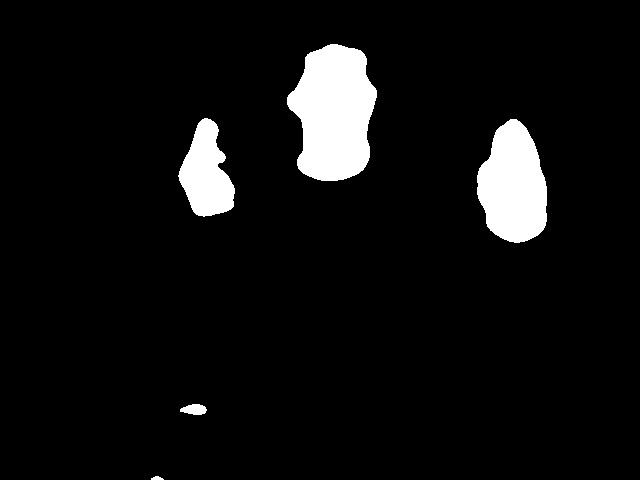
\includegraphics[width=0.5\textwidth]{figures/pipeline/thresholded.jpg}
	\caption{Thresholded image with blur preprocessing}
	\label{fig:threshold}
\end{figure}

A mechanism is required to label each pixel as skin or non-skin. The easiest way to accomplish this is by defining a threshold. All pixel values below a certain threshold are replaced with false/non-skin, all above this threshold will be replaced with true/skin. This results in a binary image with labels for (non) skin pixels. This introduces one parameter - the threshold for going from the probabilistic domain to the binary domain.

This parameter could be adjusted automatically, by comparing the percentage of skin pixels in the image and comparing this to a believed proper percentage. This percentage should be made dependent on the size of the detected face. If the percentage is too low, then the threshold should be lowered and raised if too high. 

An alternative method of going from the probabilistic domain to the binary domain is adaptive thresholding. Here the threshold is determined per pixel by the values of surrounding pixels. This method has one parameter; the neighborhood blocksize $n$ is used to determine the threshold. The threshold per pixel is calculated by the equation

\begin{eqnarray}
  \text{dst}(x, y) & \leftarrow & \left\{
  \begin{array}{l l}
	1 & \text{if src}(x,y) > T(x,y) \\
	0 & \text{otherwise} \\
  \end{array} \right.,
\end{eqnarray}

where $T(x,y)$ is the mean of the $n$ by $n$ pixel neighborhood.

\subsection*{Morphological Operations}

\begin{figure}[tb]
    \center{}
    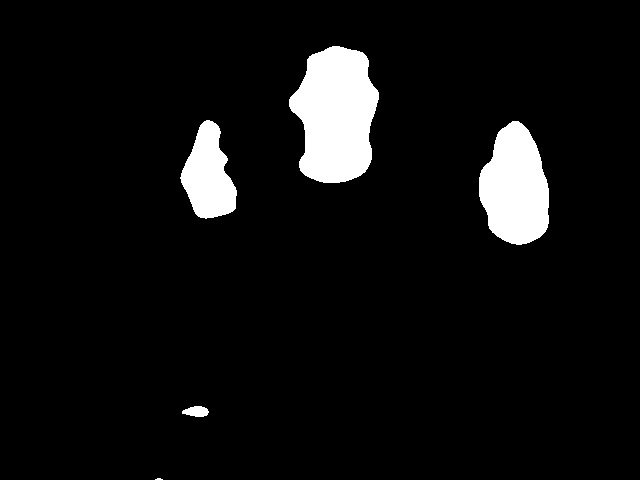
\includegraphics[width=0.5\textwidth]{figures/pipeline/closed.jpg}
	\caption{Morphologically closed}
	\label{fig:closed}
\end{figure}

An alternative to smoothing out rough edges and holes are (combinations of morphological) operations.  A morphologic closing operation of A by B is obtained by the dilation of A by B, followed by erosion of the resulting structure by B. The result of performing this operation is that small holes in the binary image are removed, and edges are smoothed as seen in \autoref{fig:closed}. The effect isn't really significant, since the gaussian smoothing already removes a lot of noise. 


\section{Object Localization}

\subsection*{Pixel Grouping, Contour Extraction}
To be able to say something useful about groups of pixels, one needs to know which pixels belong together. The human eye perceives neighboring pixels as a whole, but this is less obvious for a computer. Grouping pixels is called clustering. In this case clustering is performed by grouping pixels together that touch horizontally and vertically. Each cluster of pixels is called a blob.

To handle the blobs in a time efficient way, it is a good idea to extract the contours. In this way interesting problems can be solved efficiently like determining if a certain pixel coordinate is inside a certain blob, the maximum or minimal horizontal or vertical position and hole removal.

Since it is unusual to have holes in blobs that represent skin regions, these can be discared. This is done with the algorithm described in \citep{Suzuki1985}, where the contours of the blobs are extracted and all contours except the outer most contour are removed. This removes holes and islands in holes.

From the contours of the group, a square region of interest is defined by the outer borders. This window is called the hand window from now on.

\subsection*{Blob Labeling}

\begin{figure}[tb]
    \center{}
    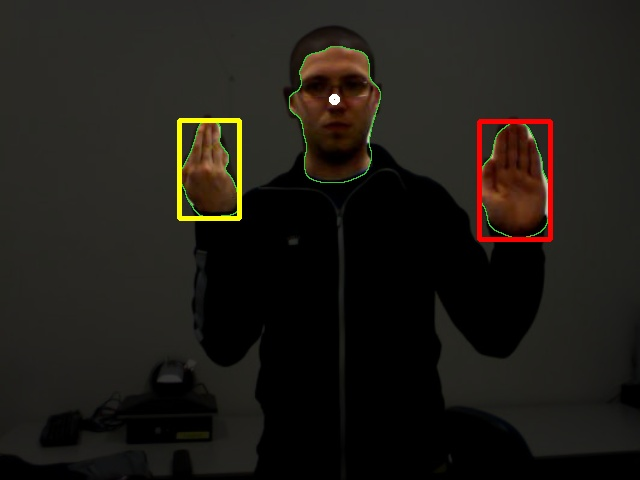
\includegraphics[width=0.5\textwidth]{figures/pipeline/contours.jpg}
	\caption{Labeled blobs with hand windows}
	\label{fig:contours}
\end{figure}

To interpret a blob the label a that blob is required. A blob can be a hand, a head or noise mislabeled as a body part. This noise can reduced by assuming a body part has a minimal size. If the surface of a blob is smaller than a certain value this blob can be discarded.

The threshold for noise is calculated by

\begin{equation}
T = (\frac{h}{c})^2,
\end{equation}

where $h$ is the height of the video in pixels and $c$ is a parameter to control the effect of the threshold. A value of $20$ for $c$ removes a lot of noise blobs, but still is small enough to leave most hand blobs intact.

Multiple cues can be used to determine which blob is which body part. The most  certain and important one is the face center, which is known as we detected the face. If a blob contains this point, this blob is the face. 

To determine which blob is which hand the relative x position to the head can be used. Algorithm \autoref{alg:blobheuristics} sorts the hands by x position and labels them with heuristics. The result of the heuristics in different scenarios is shown in \autoref{fig:heuristics}. (a) in this figure shows the usual position, where the left hand is on the left of the face and the right hand on the right. The labels are labeled accordingly. In some cases both hands are on one side of the face (b), here the relative position is used to label the hand. This is a robust method, except for the scenario where the hands positions are swapped in the x position. Fortunately this is a very unnatural body pose, so this case is just simply ignored. If such a scenario occurs the labels of the hands are mixed. 

\begin{figure}[tb]
\centering
 \subfloat[]{
   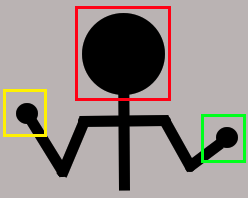
\includegraphics[width=0.29\linewidth]{figures/heurist/a.png}
}
\hspace{0.02\linewidth}
 \subfloat[]{
   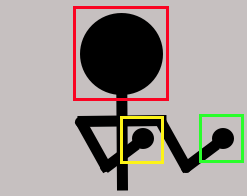
\includegraphics[width=0.29\linewidth]{figures/heurist/b.png}
}
\hspace{0.02\linewidth}
 \subfloat[]{
   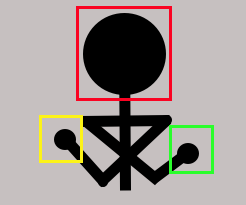
\includegraphics[width=0.29\linewidth]{figures/heurist/c.png}
}
\hspace{0.02\linewidth}
\caption{3 scenarios for ßlabeling of blobs}
\label{fig:heuristics}
\end{figure}



\begin{algorithm}
\caption{Blob labeling heuristics}
\label{alg:blobheuristics}
\begin{algorithmic}
   \REQUIRE A list of blobs `blobs'
   \REQUIRE Coordinates of a face `faceCenter'
   \ENSURE 3 or less blobs labeled head, left or right

	\FOR{blob in blobs}
		\IF{blob contains faceCenter}
			\STATE head $\leftarrow$ blob
			\STATE remove blob from blobs
		\ENDIF
	\ENDFOR

	\STATE keep only 2 biggest blobs
	\STATE sort blobs by $x$ position

	\STATE $n \leftarrow $ $|$blobs$|$
	\IF{$n = 2$}
	    \STATE left $\leftarrow$ blobs$_0$
	    \STATE right $\leftarrow$ blobs$_1$
	\ELSE
		\IF{$n = 1$}
		    \IF{center of blobs$_0$ $<$ center of face}
		        \STATE left $\leftarrow$ blobs$_0$
		    \ELSE
		        \STATE right $\leftarrow$ blobs$_0$
			\ENDIF
		\ENDIF
	\ELSE
	    \STATE no limbs found
	\ENDIF
\end{algorithmic}
\end{algorithm}



\subsection*{Blob label stabilization}
A hand doesn't move very fast in an image - usually it will not move from the left side to the right side in one frame. If this is detected this is probably a measurement error caused by noise or pour labeling. In this case the history of previous positions of a blob must be incorporated. This can be done with a Kalman Filter. A Kalman Filter is an easy and fast method for smoothing out the current position with the previous positions. The result will be a more stable estimation of the hand position. A second advantage of the Kalman Filter is the ability to actually predict the position of the hand in the next frame. This can become useful when there is no new hand detected. The hand position can then be estimated with a different method that will the the Kalman prediction.

For every hand a Kalman filter is initialized. The measurement that need to be smoothed is the hand window. The hand window has a x and y position and a width and hight. Each hand also has a speed in the x and y direction but we don't measure that - we let the kalman filter represent, calculate and use that internally. 

A hand window represented in a measurement vector as

\begin{equation}
 m_k = \left(
\begin{array}{c}
	x_k \\ %measurement.x
	y_k \\ %measurement.y,
	w_k \\ %measurement.width
	h_k \\ %measurement.height
\end{array} \right),
\end{equation}

where $x_k$ is the horizontal position, $y_k$ is the vertical position, $w_k$ is the width and $h_k$ is the height of the hand window.

The Transition matrix is defined as follows

\begin{equation}
 A = \left(
\begin{array}{cccccc}
	1 & 0 & 0 & 0 & 1 & 0 \\
	0 & 1 & 0 & 0 & 0 & 1 \\
	0 & 0 & 1 & 0 & 0 & 0 \\
	0 & 0 & 0 & 1 & 0 & 0 \\
	0 & 0 & 0 & 0 & 1 & 0 \\
	0 & 0 & 0 & 0 & 0 & 1 \\
\end{array} \right).
\end{equation}
	
This is just an identity matrix, except for the ones on the right top in the matrix. These represent the combination of the current position and the internal state of the speed.

With these matrices and a standard kalman filter the position and size of the hands can be predicted. The predicted values are used for an other hand localization method in case no hand is found en the next frame.

% setIdentity(kalman.measurementMatrix, Scalar(1));
% setIdentity(kalman.processNoiseCov, Scalar(1));
% setIdentity(kalman.measurementNoiseCov, Scalar(5));
% setIdentity(kalman.errorCovPost, Scalar(3));
% setIdentity(kalman.gain, Scalar(0e-15));
% randu(kalman.statePost, Scalar(1), Scalar(100));



% \paragraph{Update}
% The kalman filter is then updated:
% 
% Innovation or measurement residual 	
% $\tilde{\textbf{y}}_k = \textbf{z}_k - \textbf{H}_k\hat{\textbf{x}}_{k|k-1}$

% Innovation (or residual) covariance
% $\textbf{S}_k = \textbf{H}_k \textbf{P}_{k|k-1} \textbf{H}_k^\text{T} + % \textbf{R}_k$

% Optimal Kalman gain
% $\textbf{K}_k = \textbf{P}_{k|k-1}\textbf{H}_k^\text{T}\textbf{S}_k^{-1}$

% Updated (a posteriori) state estimate
% $\hat{\textbf{x}}_{k|k} = \hat{\textbf{x}}_{k|k-1} + % \textbf{K}_k\tilde{\textbf{y}}_k$

% Updated (a posteriori) estimate covariance
% $\textbf{P}_{k|k} = (I - \textbf{K}_k \textbf{H}_k) \textbf{P}_{k|k-1}$

% \paragraph{Prediction}
% And the values are predicted with:

% Predicted (a priori) state estimate 	
% $\hat{\textbf{x}}_{k|k-1} = \textbf{F}_{k}\hat{\textbf{x}}_{k-1|k-1} + % \textbf{B}_{k} \textbf{u}_{k}$

% Predicted (a priori) estimate covariance
% $\textbf{P}_{k|k-1} = \textbf{F}_{k} \textbf{P}_{k-1|k-1}
% \textbf{F}_{k}^{\text{T}} + \textbf{Q}_{k}$


\subsection*{Self Occlusion by Body Parts}
Failing to detect the hand in the current frame is caused by one of three disturbances. First of all the hand can be out of the image, or occluded by an obstacle. The second case is where the hand detection phase just fails and couldn't localize the body part. The third case is self occlusion, where the hand is very close or occluding the face or the other hand. The skin segmentation will segment this as one big blob. In this case template search is used to track the specific hand. A cut out image of the hand from the previous frame is used for this template search. Template search is a very simple and fast method, as long as the search area is small. A sliding window  with the same size as the cutout image is sliding over a small surrounding area of the location predicted by the Kalman filter. The window with the lowest squared sum difference to the previous cutout image is set as the new location. If the original cutout is touching the border of the image or the squared sum difference is too high it is assumed the hand is not visible anymore, and is flagged accordingly. This method works if the shape and size of the hand don't change too much from the last.

\begin{figure}[tb]
\begin{center}
\subfloat[detected hand]{\label{fig:template_good}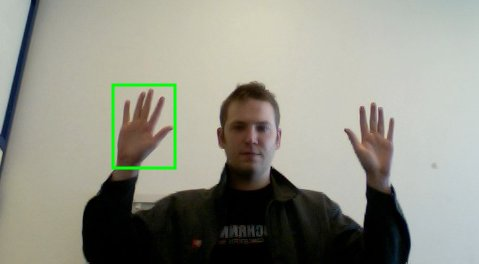
\includegraphics[width=0.45\linewidth]{figures/template/good.jpg}}
\hspace{0.03\linewidth}
\subfloat[result of template search]{\label{fig:template_occlusion}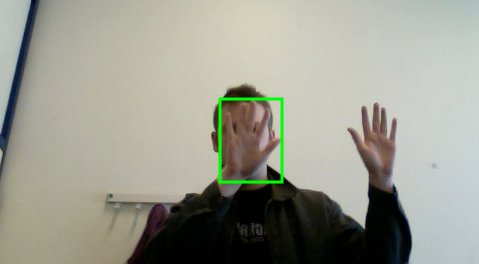
\includegraphics[width=0.45\linewidth]{figures/template/occlusion.jpg}}
\end{center}
\caption{Example of template search}
\label{fig:templatesearch}
\end{figure}

\autoref{fig:templatesearch} shows a test setting of a template search. In the left image a hand was found using the skin color model. In the second frame the hand cannot be found, because it is occluding the face and using the skin model approach the hand will be labeled as face. Using a template search the hand can still be tracked.


\section{Discussion}
This method is quite robust, but can fail if the conditions listed in \autoref{sec:goal} are not met. See \autoref{fig:fail} for an example of failed segmentation. This figure is a still from one of the movies in the dataset used in the experiments. The test subject has a skin color profile that is similar to parts of the background. Not much can be done to solve this problem, except the threshold can be manually adjusted. Still, this will introduce more false negatives and the segmentation will still be poor.

\begin{figure}[tb]
\center{}
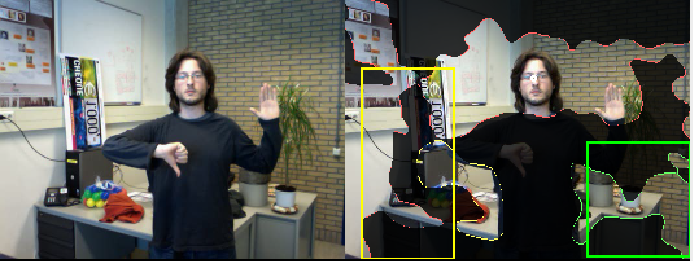
\includegraphics[width=0.8\linewidth]{figures/fail.png}
\caption{Example of failed segmentation}
\label{fig:fail}
\end{figure}

Thresholding can be adjusted automatically by adaptive thresholding. The downside of the method is that it requires a large neighborhood value to work in a reasonable stable way, which becomes to computationally expensive. Also, the background will be clustered as a blob also, which introduces an extra blob removal step. \autoref{fig:thresholdedAdap} shows the example output of a adaptive threshold with a neighborhood of 51.


\begin{figure}[tb]
\center{}
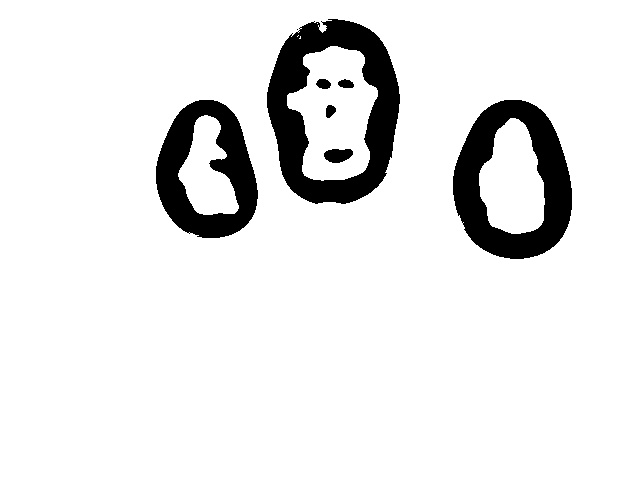
\includegraphics[width=0.3\linewidth]{figures/pipeline/thresholdedAdap.jpg}
\caption{Adaptive threshold with pixel neighborhood of 51}
\label{fig:thresholdedAdap}
\end{figure}






